\chapter{Error Analysis via Simulation}\label{ch:simulation}
% word checked.
The flight test result proved the feasibility of using CC\_EKF\_SLAM
algorithm for distance object mapping. It also revealed there existed
some error in the result of the algorithm, with error of up to 30
meters for SUAS localization and up to 150 meters for most landmarks
positions. It is important to understand the cause of these errors so
that improvement on the algorithm can be made.

There are many factors affecting the accuracy in UAV localization and
landmarks mapping results, and they can be sorted into three main
categories:

\begin{enumerate}
  \item Error caused by the SLAM algorithm itself. The algorithm
  estimated landmarks coordinates through a model that describes the
  relation between the UAV and landmarks. As the model is non-linear,
  the linearization process introduces error into the result.
  \item Noise in system intrinsic parameters. The system intrinsic
  parameters include
  \begin{itemize}
    \item Camera intrinsic parameters
    \begin{itemize}
      \item Coordinate of optical center on image plane $[c_{x}, c_{y}]$
      \item Scaling factors that project landmarks in 3D world to image plane $ [f_{x}, f_{y}]$
      \item Lens distortion parameters $[k_{1}, k_{2}, p_{1}, p_{2}]$
    \end{itemize}
    \item Image resolution.
    \item Accelerometer bias % expand
  \end{itemize}
  \item Error introduced by Lucas-Kanade (LK) tracking algorithm. LK
  tracking algorithm tracks landmarks by comparing the intensity of a
  windowed image centered at the landmark coordinate from one frame to
  another. The searching of matching window terminates when the sum of
  squared error (SSE) on the windowed image is lower than a threshold
  set by user, or when the number of iteration of the search has
  reached a maximum number (also set by user). As scene evolves from
  frame to frame, the initial landmark appears differently as viewing
  distance and angle changes. Allowing a small SSE between matched
  windows is necessary to give tolerance for the matching. However, it
  could also cause the window to move in the neighborhood of the
  landmark coordinate, and eventually drift off, resulting in a loss
  of the original landmark. An example was shown in figure
  \ref{fltfig:1_1} in chapter \ref{ch:FlightResult}. Secondly, sudden
  intensity change in image sequences could result in significant
  noise in the tracking. In outdoor setting, intensity change can be
  introduced by many factors, such as changes of sky portion in an
  image, sun glare, UAV entering or exiting cloud shades, or camera
  auto-adjusting its shutter speed, etc. As reliable vision tracking
  algorithm is an entire field of research in itself, it will not be
  discussed further in this chapter.

\end{enumerate}

To better understand the impact from the noise of system intrinsic
parameters listed above. A simulation was performed to examine item 1
and 2. The simulator first generated a 3D point cloud ranging between
100 meters to 1500 meters from the camera (Figure \ref{fig:simfig51}).
At each frame, the coordinates of the 3D points were first transformed
to the new camera frame using a simulated UAV pose, which allows for
studying the algorithm under various motion. Next, the 3D points were
projected onto the image plane using a camera model defined by
$[c_{x}, c_{y}, f_{x}, f_{y}, k_{1}, k_{2}, p_{1}, p_{2}]$, and
digitized to a resolution of choice. The resulting coordinates of the
3D points were used directly as measurement in the update of the EKF.
The procedure described above simulated the entire process of
perceiving landmark through a digital camera under arbitrary UAV
motion. What it does not simulate is error contributed by visual
tracking algorithm, and by navigation measurements.

\begin{figure}[h]
\centering
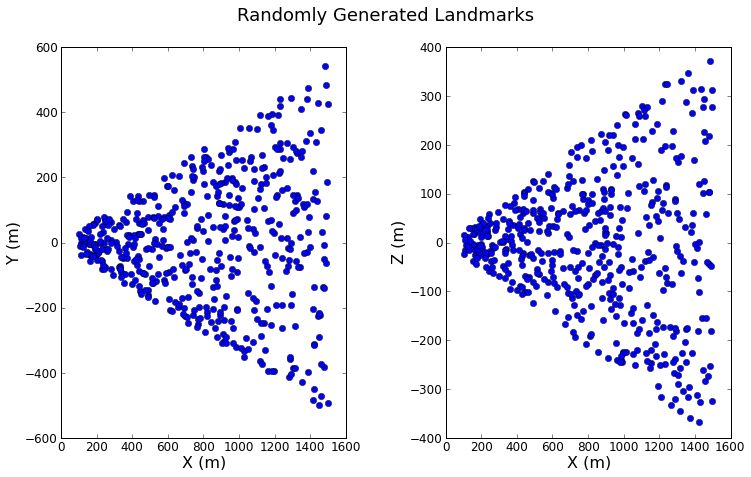
\includegraphics[width=12cm, height=7cm]{./Figures/SimulationFigures/Figure51.png}
\caption{Randomly Generated 3D Landmark Points}
\label{fig:simfig51}
\end{figure}
\FloatBarrier

\section{An Ideal Case}
% word checked.
First of all, understanding the algorithm's performance under nearly
no noise condition provides a solid ground for the analysis later on.
This simulation showed how much error the model itself generated under
the most basic flying condition, which is moving forward at constant
speed. The low noise environment was configure as such,

\begin{itemize}
  \item UAV was moving forward (X axis) with constant speed at 60 knots. 
  \item Y axis and Z axis translation were limited to white noise with
  standard deviation of 0.08 meters and a mean of 0.
  \item UAV rotation were modelled by white noise with standard
  deviation of 0.01 degree and a mean of 0 degree.
  \item No image digitization (i.e. the projected landmark position on
  image plane was not digitized to any sensor resolution)
  \item No error was introduced from camera model mismatch (i.e.
  camera intrinsic parameters used by the simulator was exactly the
  same as those used in CC\_EKF\_SLAM algorithm.
\end{itemize}

\subsection{UAV Localization}
% word checked.
UAV poses were plotted in Figure \ref{fig:simfig1}. The ground truth
and estimated value were plotted in blue and green lines respectively.
The error was plotted in red line. Under a simple forward only motion,
the algorithm tracked the UAV status quite well. Error on
translational motion was less than 1 cm and error on rotational motion
less than 3e-3 degree. An obvious behavior of the error is that the
error started from 0, experienced some rapid change during the first
few frames, and settled to a relatively stable value. This matched the
converging behavior of the landmark inverse depth $\rho$ which was
shown next. This observation suggested that although inverse depth
representation is more linear than direct depth representation, it has
a negative impact on the accuracy of the estimates when being included
in the filter vector before its approximate value is known. Hence,
delaying integration of inverse depth till its value is approximately
known should increase the accuracy of the state vector estimates. As
triangulating a landmark requires 2 frames in monocular vision setup,
the delay requires only one extra frame, and is insignificant in most
scenario.

\begin{figure}[h]
\centering
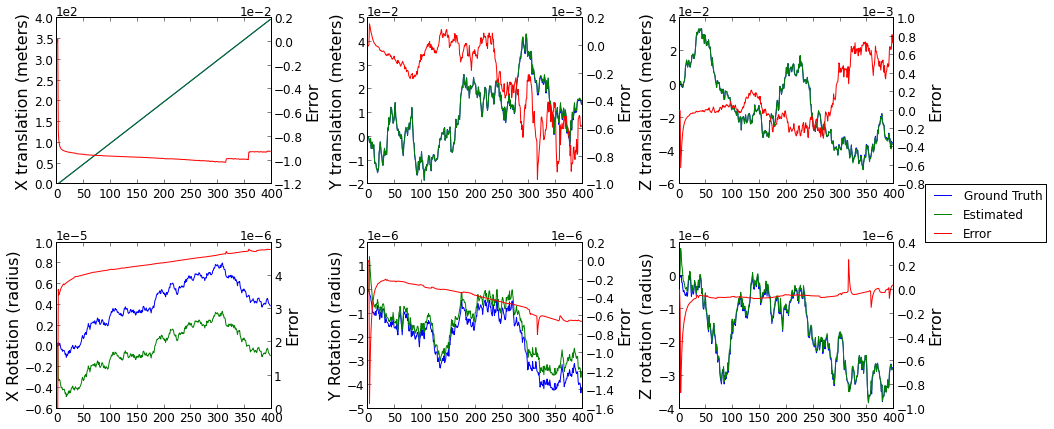
\includegraphics[width=16cm, height=8cm]{./Figures/SimulationFigures/Figure1.png}
\caption{UAV localization error under no noise condition}
\label{fig:simfig1}
\end{figure}
\FloatBarrier

\subsection{Landmarks Mapping - Convergence and Accuracy}
% word checked.
Figure \ref{fig:simfig5-8} top left showed landmark parameters $[d,
\varphi ,\theta]$ (where $d=1/\rho $) plotted against frame number for
the first 50 frames. The landmark depth $d$ for all landmarks
converged within the first 3 frames. The elevation-azimuth angles
$[\varphi ,\theta]$ stayed almost constant after initialization. More
detail can be seen from the error convergence plot for these
parameters, plotted in Figure \ref{fig:simfig5-8} top right. The error
of landmark distance $d$ slowly converged to zero as the tracking
continued. $[\varphi ,\theta]$ errors started from 0 at frame 0, and
converged to a small offset while landmark depth $d$ converged. As
discussed in chapter \ref{ch:FlightResult}, in order to compensate for
the inaccurate estimates on depth at filter initialization, the EKF
made adjustment to $\varphi$ and $\theta$ so that the resulting
coordinates of landmarks agreed with the measurement. Therefore early
integration of landmark depth had negative impact on the estimates
accuracy. 

\begin{figure}[h]
\centering
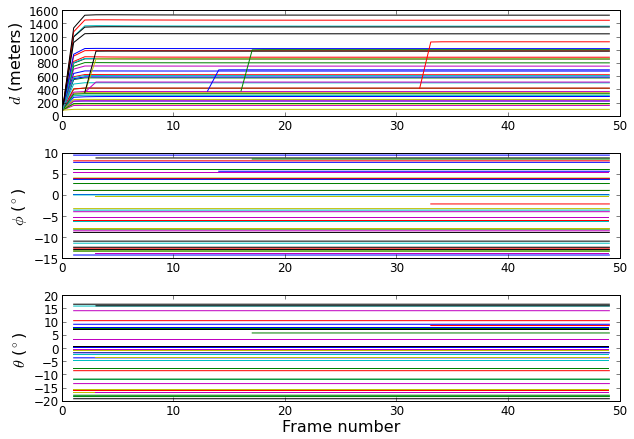
\includegraphics[width=7cm, height=5cm]{./Figures/SimulationFigures/Figure6.png}
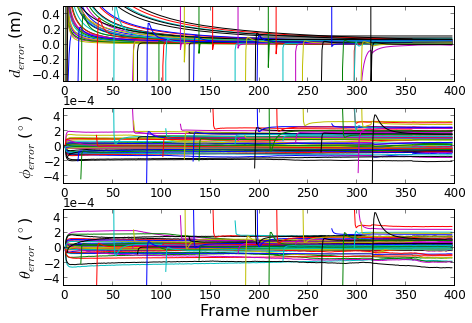
\includegraphics[width=7cm, height=5cm]{./Figures/SimulationFigures/Figure7.png}
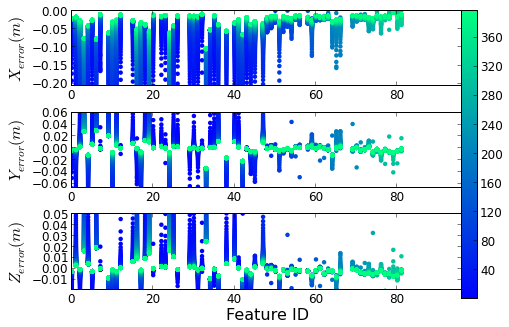
\includegraphics[width=7cm, height=5cm]{./Figures/SimulationFigures/Figure5.png}
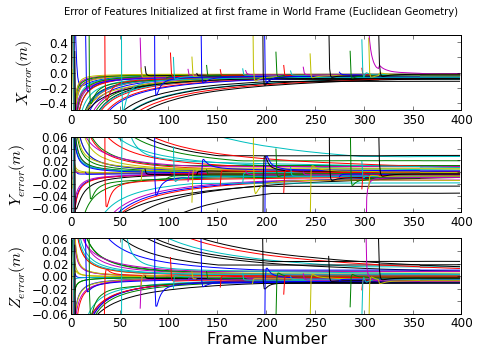
\includegraphics[width=7cm, height=5cm]{./Figures/SimulationFigures/Figure8.png}
\caption{Landmarks parameters and error convergence under low noise condition}
\label{fig:simfig5-8}
\end{figure}

The error for landmarks coordinates in world frame were plotted
against landmark ID and frame number in figure \ref{fig:simfig5-8}
bottom left and right. The landmarks coordinates errors in world frame
all converged toward zero. During the 400 frames period, some
landmarks moved out of the FOV, and therefore their position estimates
remained unchanged since then. At the end of the 400 frames, landmarks
coordinates error on x axis reduced to +/-0.2 meters; on y and z axis,
errors reduced to +/-0.02 meters. In summary, factors that cause
error in landmarks positions were listed below. 

\begin{itemize}
  \item Error in UAV localization caused an offset error when new
  landmark was added to the filter.
  \item Early landmark integration caused offset error in $\varphi$
  and $\theta$ estimates due to EKF compensating for landmark depth at
  integration.
  \item Some landmark moved out of FOV before fully converged.
\end{itemize}
\FloatBarrier

\section{Effect of Motion}
% word checked.
The simulation result from UAV forward travel showed that the
CC\_EKF\_SLAM algorithm does landmark tracking and self localization
quite well under simple motion. Next, the algorithm was tested with a
more complex and realistic scenario. A series of motion was added to
the simulation in addition to the forward motion. The remaining 5
types of maneuvers were examined independently. These maneuvers are:
translation on Y, translation on Z, rotation on X, rotation on Y and
rotation on Z. As motions on all other 5 D.O.F. are mostly oscillatory
when the UAV moves forward, each motion was modelled by a Sine wave
with frequency at 1Hz and variable amplitude. 

$$\text{Added motion} = A_{\text{motion type}}\cdot sin(2\pi x+\pi/2)$$

Motion type is denoted by $v_y$, $v_z$ for translation on Y and Z
axes; $w_x$, $w_y$ and $w_z$ for rotation on X, Y, and Z axes. For
translation, the Sine amplitude $A_{v_y,v_z}$ varied from 1 meter to
19 meters with 2 meters increment. For rotation, the amplitude
$A_{w_x,w_y,w_z}$ varied from 0.001 radius to 0.018 radius
(0.057$^\circ$ to 1.031$^\circ$) with 0.001 radius increment.

\subsection{UAV Localization under Motion}\label{localization_motion}

Figure \ref{fig:simfig9-10} showed the UAV localization error
statistic under oscillatory translation on Y and Z axis and
oscillatory rotation on X, Y, and Z axis. The blue dots marked the mean
value $\mu$ of the error throughout 400 frames of tracking, and the
error bars marked the standard deviation $\sigma$.

The translation motion clearly increased the error of UAV
localization. However, the amount was insignificant. With the Sine
amplitude increased to 19m, UAV position error increased by less than
0.02 meter.

On the other hand, rotational motions had a big impact on the accuracy
of localization. Rotation on X axis (roll) had small effect. No
obvious increase on mean and standard deviation can be
observed. Rotations on Y and Z axis yielded significant error.

\begin{itemize}
  \item Rotation on Y axis increased the mean and standard deviation
  of UAV position error on X. For UAV position on Z, the mean
  error stays zero, but standard deviation increased dramatically.
  \item The same behavior can be observed on the X and Y axes position
  error for rotation on Z axis.
\end{itemize}

\begin{figure}[h]
  \centering
  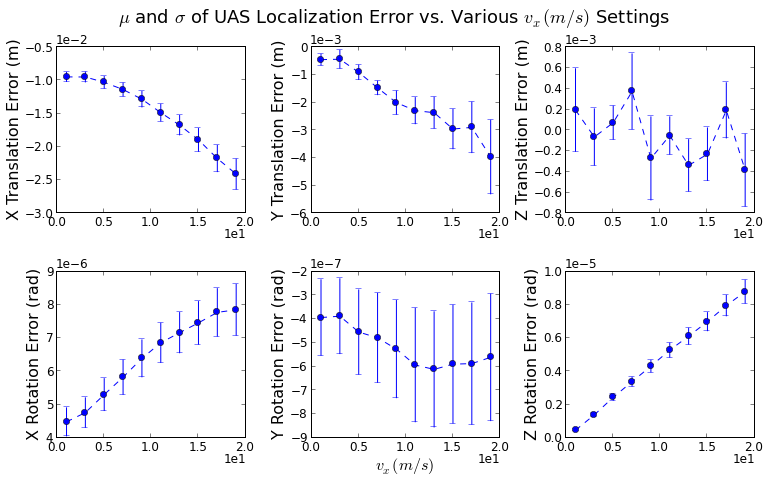
\includegraphics[width=7cm, keepaspectratio=true]{./Figures/SimulationFigures/Figure9.png}
  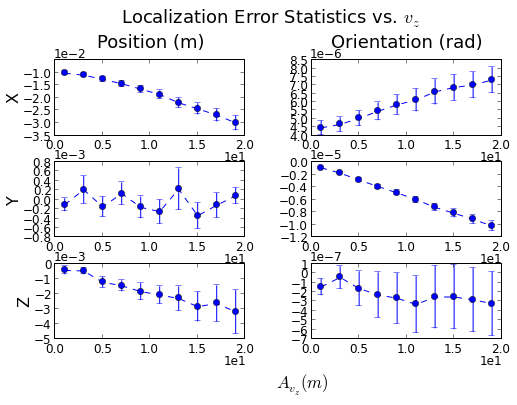
\includegraphics[width=7cm, keepaspectratio=true]{./Figures/SimulationFigures/Figure10.png}
  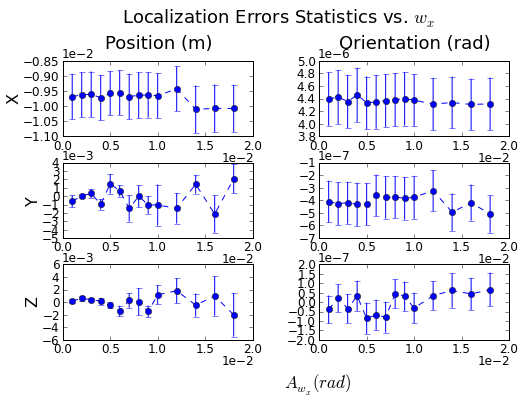
\includegraphics[width=7cm, keepaspectratio=true]{./Figures/SimulationFigures/Figure11.png}
  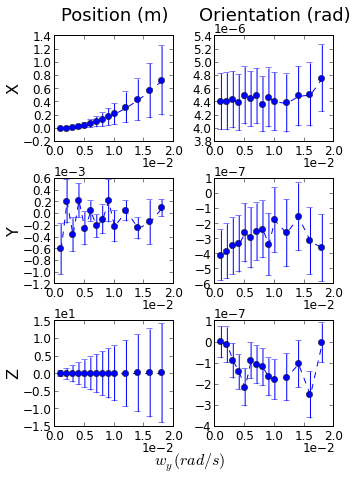
\includegraphics[width=7cm, keepaspectratio=true]{./Figures/SimulationFigures/Figure12.png}
  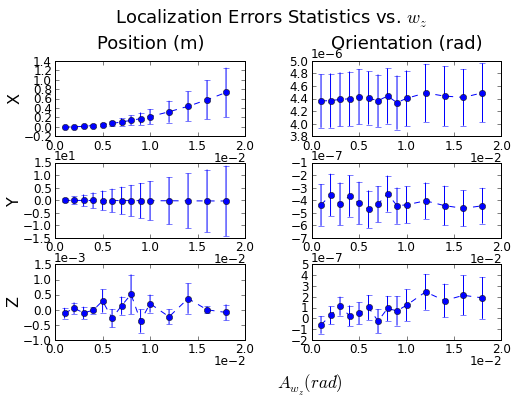
\includegraphics[width=7cm, keepaspectratio=true]{./Figures/SimulationFigures/Figure13.png}
  \caption{UAV localization errors under translational 
  \label{fig:simfig9-10}
    motion}
\end{figure}
\FloatBarrier

To understand how rotation affected the UAV localization estimates,
UAV positions on X, Y, Z in world frame were plotted below (figure
\ref{fig:simfig14}) with rotation Sine amplitude on X, Y and Z set at
0.01 radius. When rotation occurred on X axis, the position error of
the UAV showed some oscillation. The oscillation magnitude remained
small (in the scale of millimeters) and around zero, hence, did not
generate significant mean and standard deviation change on the error
statistic plot. For rotation on Y and Z, increase of rotational motion
caused an increasing oscillatory error on the UAV position estimates
(diverging). The mean error on UAV X-axis position increased in
positive value with rotational motion on both Y and Z axes. The most
significant impact happened on the Z-axis position (for rotation on
Y) and Y-axis position (for rotation on Z), with error reaching 20
meters peak-to-peak at the end of the 400 frames. With an increasing
rate of rotation (amplitude of the Sine wave), the rate of error
diverging from zero also increased, hence, resulting in an increasing
error standard deviation in the error statistic plots. This simulation
result suggested that CC\_EKF\_SLAM algorithm is very sensitive to
rotational motion on Y and Z axes.

\begin{figure}[h]
  \centering
  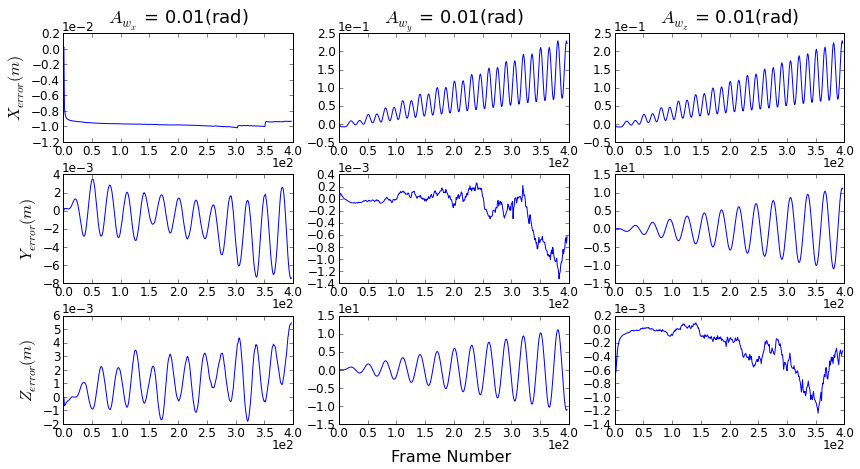
\includegraphics[width=13cm, keepaspectratio=true]{./Figures/SimulationFigures/Figure14.png}
  \caption{Estimated UAV position in world frame with rotational
    motion on Y and Z axes set at 0.01 rad/s}
  \label{fig:simfig14}
\end{figure}
\FloatBarrier

\subsection{Landmark Mapping Accuracy under Motion}\label{sec:landmarkMotion}
% word checked.
Landmark mapping error statistics were calculated from the landmark
errors at the last frame. Figure \ref{fig:simfig20-24} showed the
landmark mapping error statistics with added motions. 

Translational motions increased both the mean and standard deviation
of landmark mapping errors, but not by much. With the motion maximum
amplitude ranging from 1 meter to 19 meters, the increases on mean and
standard deviation were both in the scale of centimeters.

\begin{figure}[h]
  \centering
  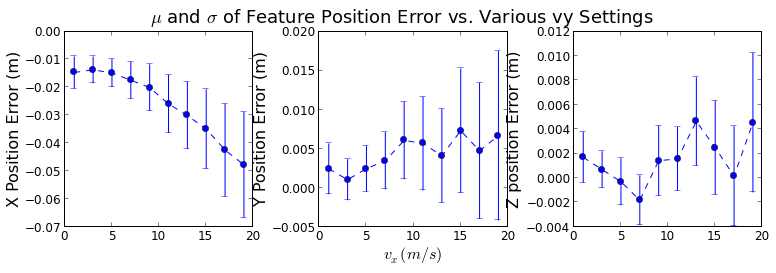
\includegraphics[width=10cm, keepaspectratio=true]{./Figures/SimulationFigures/Figure20.png}
  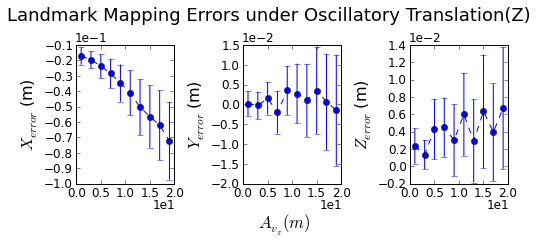
\includegraphics[width=10cm, keepaspectratio=true]{./Figures/SimulationFigures/Figure21.png}
  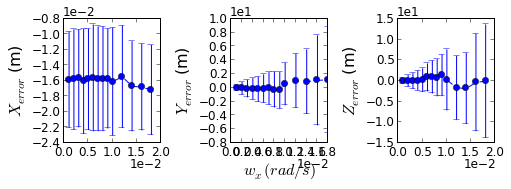
\includegraphics[width=10cm, keepaspectratio=true]{./Figures/SimulationFigures/Figure22.png}
  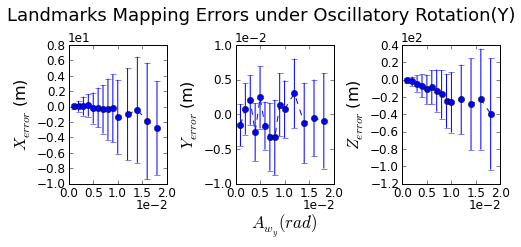
\includegraphics[width=10cm, keepaspectratio=true]{./Figures/SimulationFigures/Figure23.png}
  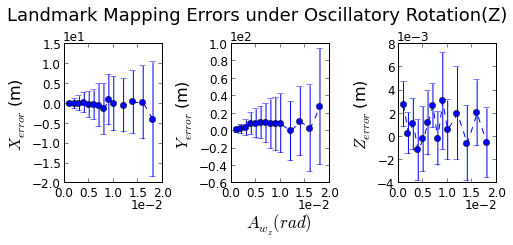
\includegraphics[width=10cm, keepaspectratio=true]{./Figures/SimulationFigures/Figure24.png}
  \caption{Landmark mapping error under added motion}
  \label{fig:simfig20-24}
\end{figure}

Rotational motion had much bigger effect on the accuracy. With
amplitude of Sine wave rotation ranging from 0.001 radius to 0.018
radius (0.057$^\circ$ to 1.031$^\circ$)

\begin{itemize}
  \item X axis rotation caused a small standard deviation increase on
  the errors of landmarks positions on Y and Z axes. The errors were in the
  scale of meters under maximum rotation setting.
  \item Y axis rotation caused mean and standard deviation increase on
  the errors of landmarks positions on X and Z axes. Landmarks positions on Z
  received the biggest impact with error in the scale of hundreds of
  meters under maximum rotation setting.
  \item Z axis rotation affected landmark mapping on X and Y axes in a
  similar way as the Y axis rotation did.
\end{itemize}
\FloatBarrier
\begin{figure}[h]
  \centering
  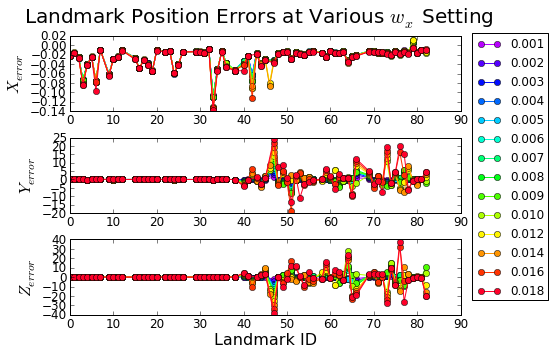
\includegraphics[width=7cm, height=5cm]{./Figures/SimulationFigures/Figure17.png}
  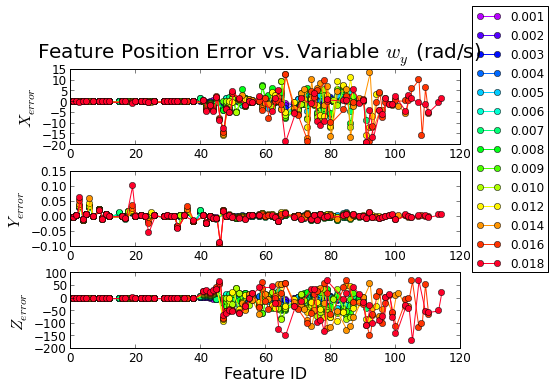
\includegraphics[width=7cm, height=5cm]{./Figures/SimulationFigures/Figure18.png}
  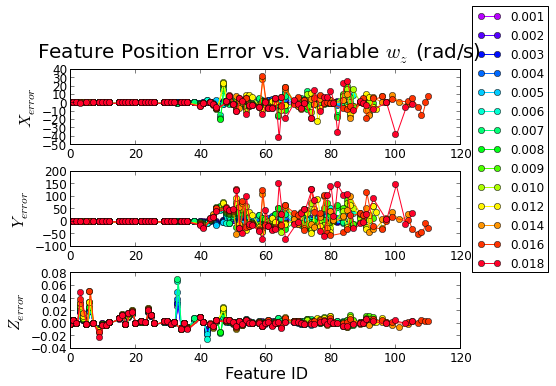
\includegraphics[width=7cm, height=5cm]{./Figures/SimulationFigures/Figure19.png}
  \caption{Landmark mapping error under rotational motion}
  \label{fig:simfig17-19}
\end{figure}

Figure \ref{fig:simfig17-19} showed landmarks positions errors at
the last frame plotted against landmark IDs (initialization
sequence), with line and marker color indicating various rotation setting.

\begin{itemize}
  \item With rotation on Y and Z, tracked landmarks were easily lost
  as they went out of FOV. This can be observed from from landmark ID
  increasing from 80 to over 110 with Y axis rotation setting varied
  from 0.001rad to 0.018rad. A frequent addition of new landmark
  has negative impact on the overall result due to the correlation
  between landmarks. 
  \item Landmarks added after first frame has much bigger error than
  landmarks added at first frame. At 1$^{st}$ frame, 40 landmarks were
  added to the filter. All three plots in figure \ref{fig:simfig17-19}
  showed that major landmark mapping error came from landmarks added
  after the 1 $^{st}$ frame with ID bigger than 40.
\end{itemize}
\FloatBarrier

To investigate how rotational motion resulted in bigger error on
landmarks added after first frame, the scenario of UAV experiencing
rotation on Y-axis with $A_{w_y}=0.01rad$ was analyzed. Landmarks
parameters were converted into world frame and their error were
plotted in figure \ref{fig:simfig25}. It was found that the most
significant error occurred on parameter $\varphi$ which is the landmark
elevation angle. This angle has the same definition as rotation angle
around Y axis. The second biggest contributor was $z_i$, the landmark
initialization coordinate on Z axis. Both parameters $\varphi$ and
$z_i$ had offset error at initialization, and were never corrected
throughout the tracking.

Regarding the offset error in $z_i$, as discussed in section
\ref{localization_motion}, UAV localization estimates had the biggest
position error on X and Z axes under Y-axis rotation. All landmarks
not initialized at $1^{st}$ frame would be affected by the UAV
localization error, since the initialization point and UAV position
are correlated.

\begin{figure}[h]
  \centering
  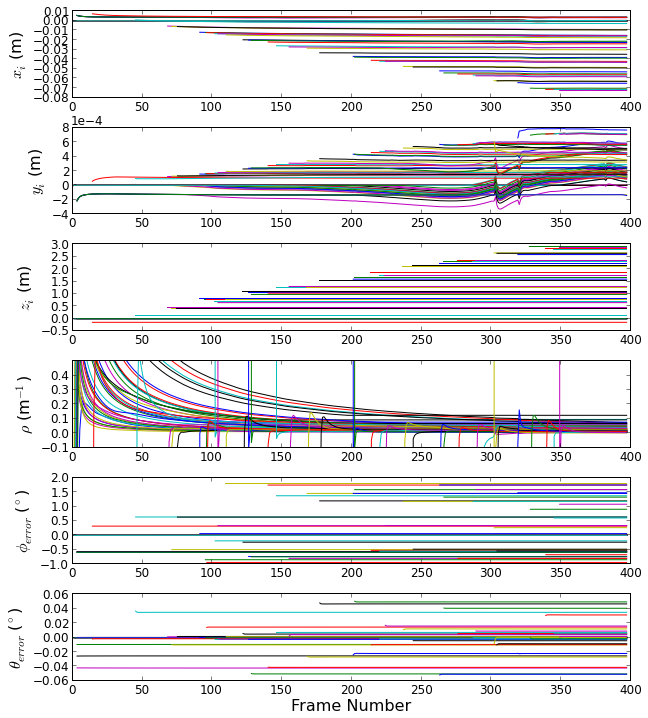
\includegraphics[width=10cm, height=12cm]{./Figures/SimulationFigures/Figure25.png}
  \caption{Landmark parameters error under rotational motion on
    Y-axis, $A_{w_y}=0.01rad$}
  \label{fig:simfig25}
\end{figure}
\FloatBarrier

Figure \ref{fig:simfig26} showed the $\varphi$ error at initialization
in camera frame and world frame. The blue line showed error in camera
frame. The red line showed error in world frame transformed using the
estimated UAV position and orientation. As $\varphi$ error was nearly
0 in camera frame, it is clear that the reference frame transformation
introduced the offset error. During reference frame transformation,
ground truth landmarks were transformed using the ground truth UAV
poses; estimated landmark were transformed using estimated UAV poses.
Hence, even though the parameters were the same in camera frame,
result in world frame would be different. Landmarks initialized at the
first frame didn't carry any offset error because the reference frame
transformation was using the same parameters in both way. During
tracking, these landmarks were transformed to the new camera frame
using the estimated UAV position and orientation. These were the same
values being used to transform landmark position from camera frame
back into world frame. Therefore, although the UAV localization
estimates were different from the ground truth, landmark initialized
at first frame were not affected. 

To conclude, the main contributor for landmark mapping error came
from error in UAV localization estimation.

\begin{figure}[h] %redo figure, change phi to varphi
  \centering
  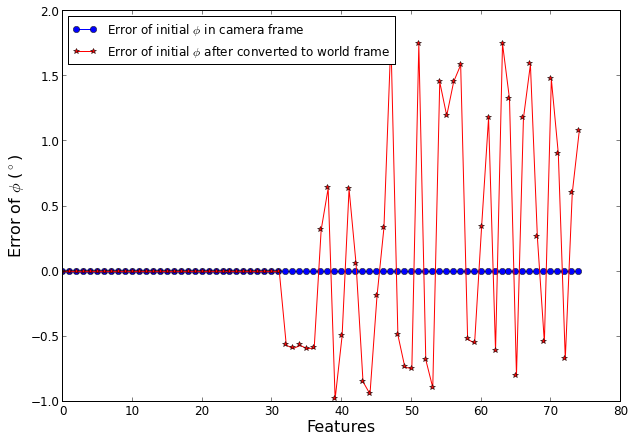
\includegraphics[width=10cm, height=7cm]{./Figures/SimulationFigures/Figure26.png}
  \caption{Error of $\varphi$ in camera frame and world frame at initialization}
  \label{fig:simfig26}
\end{figure}
\FloatBarrier

\section{Camera Intrinsic Parameters}
% word checked.
This section discussed the effect on CC\_EKF\_SLAM accuracy from
calibration error of camera intrinsic parameters. Errors on camera
intrinsic parameters were simulated by using different values in the
camera models used by the simulator and by the CC\_EKF\_SLAM algorithm.
$c_{x}$, $c_{y}$, $f_{x}$, and $f_{y}$ were simulated individually and
distortion parameters $[k1, k2, p1, p2]$ were simulated as a group.
Using the calibrated camera model (see section \ref{sec:camcal}) as a
base model, $c_{x}$, $c_{y}$, $f_{x}$, and $f_{y}$ in simulator
camera model varied from -50\% to 50\% of the base model. Distortion
parameters varied from 0\% to 140\% of the base model.

\subsection{Effect from $(c_{x}, c_{y})$}
% word checked.
Figure \ref{fig:simfig34-35} showed an overview of UAV poses error
statistics with $(c_{x}, c_{y})$ calibration error introduced. From
the statistic plot, it was found that $c_x$ had biggest impact on UAV
position on X and Y, and $c_y$ had biggest impact on UAV position on X
and Z.

\begin{figure}[h]
  \centering
  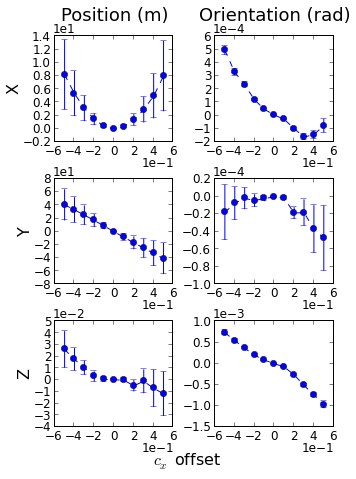
\includegraphics[width=7cm, keepaspectratio=true]{./Figures/SimulationFigures/Figure34.png}
  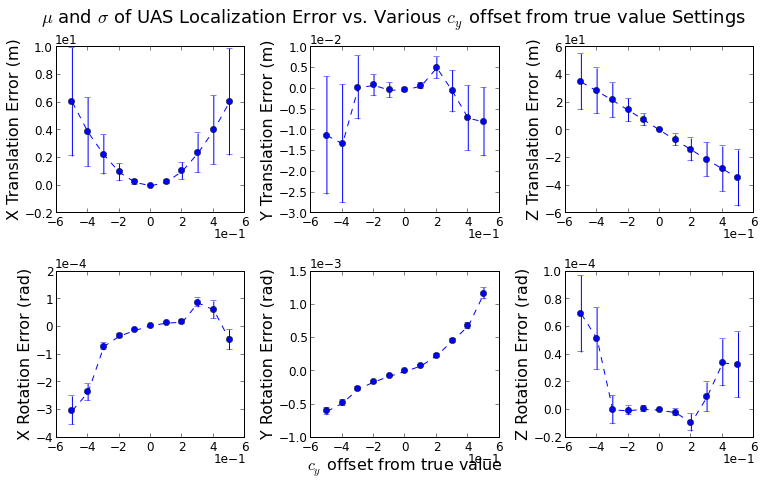
\includegraphics[width=7cm, keepaspectratio=true]{./Figures/SimulationFigures/Figure35.png}
  \caption{UAV localization error statistics with varying $(c_x, c_y)$}
  \label{fig:simfig34-35}
\end{figure}

Figure \ref{fig:simfig36-37} showed the UAV position error with $c_x$
and $c_y$ at various offset from the base value. The resulted UAV
positions errors were dependent on both $(c_{x}, c_{y})$ and were
divergent in time. The divergence can be modeled by 1$^{st}$ order
polynomial function, with the rate of divergence decided by the offset
of $(c_{x}, c_{y})$ from the base value.

\begin{figure}[h]
  \centering
  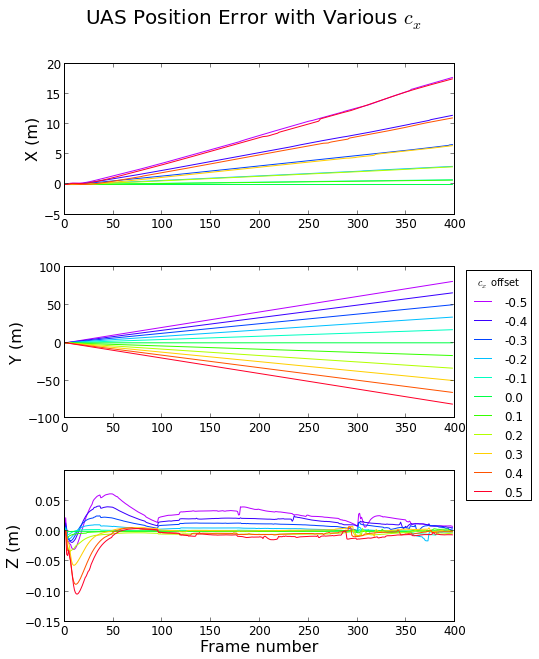
\includegraphics[width=7cm,keepaspectratio=true]{./Figures/SimulationFigures/Figure36.png}
  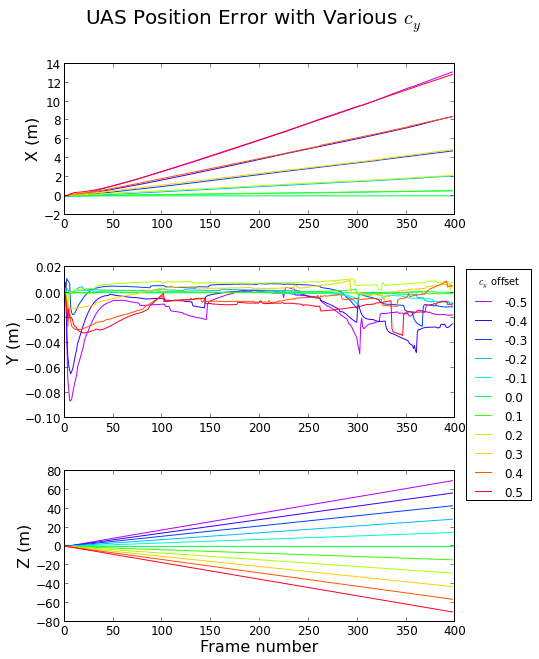
\includegraphics[width=7cm,keepaspectratio=true]{./Figures/SimulationFigures/Figure37.png}
  \caption{Diverging UAV position error}
  \label{fig:simfig36-37}
\end{figure}
\FloatBarrier

The landmarks mapping errors statistics from calibration error of
$(c_{x}, c_{y})$ were plotted in figure \ref{fig:simfig28-29}. The
following characters can be observed from the plots:

\begin{itemize}
  \item Calibration error on $c_{x}$ affected landmarks positions on all
  axes, among which, X and Y axes showed the most significant error.
  \begin{itemize}
    \item The further $c_{x}$ deviated from the base value, the further
    the landmarks appeared in average (positive mean error on X).
    \item Mean landmarks positions errors on Y axis was proportional to
    the calibration error on $c_x$. Their relation can be modeled by
    1$^{st}$ degree polynomial equation.
    \item Error on $c_{x}$ also affected landmarks positions on Z
    axis, but in the scales of a few meters.
  \end{itemize}
  \item Calibration error on $c_{y}$ affected landmarks positions on
  all axis similarly to $c_{x}$. Estimates on X and Z axes showed the
  most amount of error.
\end{itemize}

\begin{figure}[h] % change plots title to "Landmarks Mapping Errors
                  % Statistics
                  % and C_x/C_y offset
  \centering
  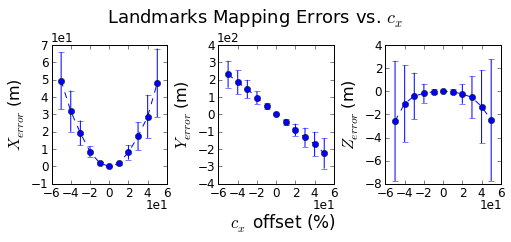
\includegraphics[width=10cm, keepaspectratio=true]{./Figures/SimulationFigures/Figure28.png}
  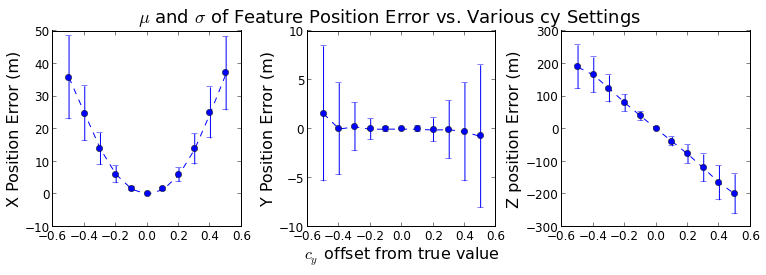
\includegraphics[width=10cm, keepaspectratio=true]{./Figures/SimulationFigures/Figure29.png}
  \caption{Landmarks mapping errors statistics with varying $(c_x, c_y)$}
  \label{fig:simfig28-29}
\end{figure}

Plotting landmarks positions errors against landmarks ground truth
positions revealed more information on how $c_{x}$ and $c_{y}$
affected landmark mapping. Landmarks positions errors were dependent
on their ground truth positions, and $c_{x}$ (or $c_{y}$).

\begin{itemize}
  \item Landmarks positions errors on X axis were proportional to the
  landmarks ground truth positions on X. The further the landmark was,
  greater the error would be. The amount of incorrectness in $c_{x}$
  decided the slope of the error plot. The greater the error was in
  $c_{x}$, the steeper the slope became (figure \ref{fig:simfig32-33} left,
  subplot $[1,1]$).
  \item Landmarks positions errors on Y axis were also proportional to
  their ground truth positions on X with the slope steepness and
  polarity dependable on the amount and polarity of the error of
  $c_{x}$ (figure \ref{fig:simfig32-33} left, subplot $[2,1]$).
  \item Landmarks positions errors on Z axis were proportional to
  their ground truth positions on Z, with slope steepness and polarity
  dependable on the amount and polarity of error of $c_{x}$ (figure
  \ref{fig:simfig32-33} left, subplot $[3,3]$).
\end{itemize}

$c_{y}$ affected landmarks positions similarly to $c_{x}$ (figure
\ref{fig:simfig32-33}, right).

\begin{figure}[h]
  \centering
  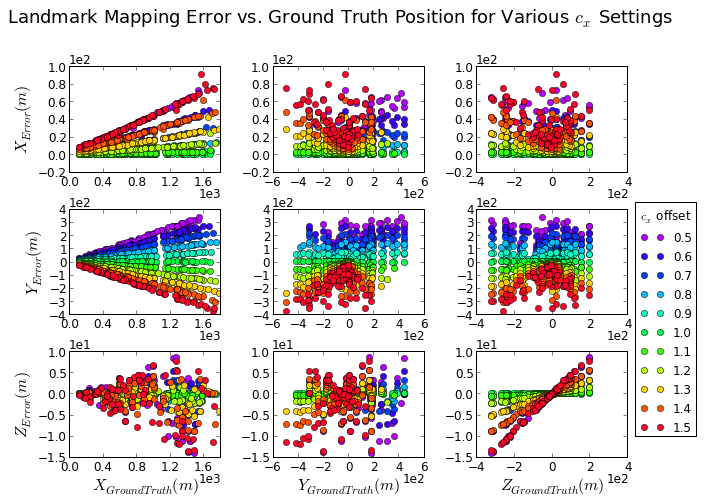
\includegraphics[width=13cm, keepaspectratio=true]{./Figures/SimulationFigures/Figure32.png}
  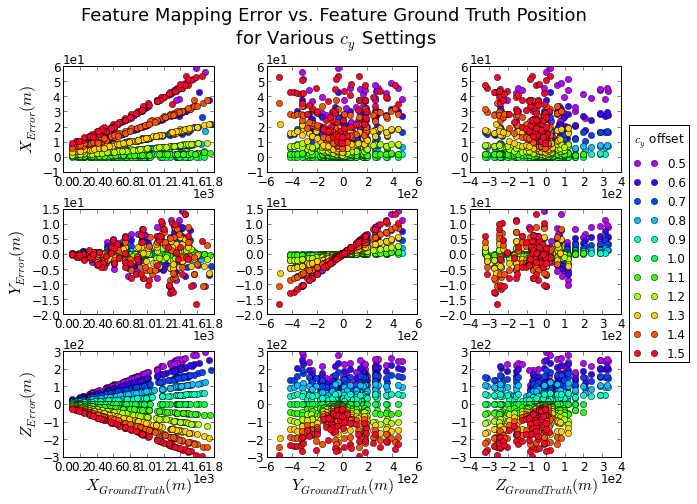
\includegraphics[width=13cm, keepaspectratio=true]{./Figures/SimulationFigures/Figure33.png}
  \caption{Landmarks mapping errors vs. ground truth landmarks positions}
  \label{fig:simfig32-33}
\end{figure}
\FloatBarrier

\subsection{Effect from $(f_x, f_y)$}

With $(f_x, f_y)$ varying from -50\% to +50\% of the base value, the
UAV localization errors were shown in \ref{fig:simfig43-44}. For all
$f_x$ and $f_y$ settings, UAV position errors remained less than
+/-0.05 meters, and orientation errors remained less than 8e-6 radius.
Compared to the errors obtained from the ideal case, calibration
errors in $(f_x, f_y)$ did not introduce any additional error into UAV
localization estimates.
\begin{figure}[h]
  \centering
  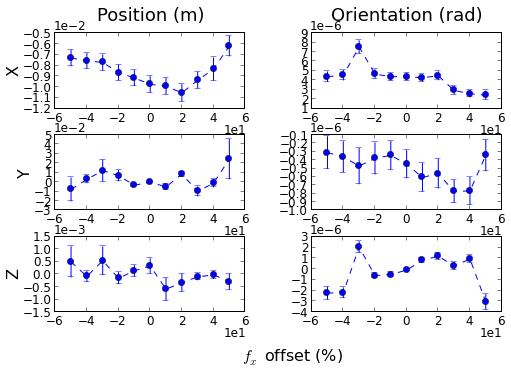
\includegraphics[width=7cm,keepaspectratio=true]{./Figures/SimulationFigures/Figure43.png}
  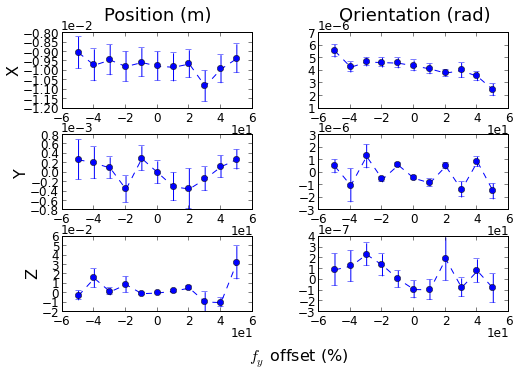
\includegraphics[width=7cm,keepaspectratio=true]{./Figures/SimulationFigures/Figure44.png}
  \caption{UAV localization errors statistic with variable $(f_x, f_y)$}
  \label{fig:simfig43-44}
\end{figure}

On the other hand, landmarks mapping errors were unavoidably affected
by the calibration errors in $(f_x, f_y)$ since these were the scaling
factors that projected landmarks from 3D world onto image plane.
Figure \ref{fig:simfig38-39} showed the errors statistics of landmarks
positions estimates under various $(f_x, f_y)$ settings. The effect on
the X axis was minimal and was in the scale of millimeter. Errors on Y
axis received the most impact from error on $f_x$, since this was the
scale factor that mapped the Y component of landmarks position in
world onto u-axis on image plane by $u = Y/X \cdot f_x$. Same behavior
happened on the landmarks positions estimates on Z axis and their
relation to $f_y$.

\begin{figure}[h]% Change title to "Landmarks mapping Errors
                 % Statistics and Projection Scalling Factor (f_x/f_y)
  \centering
  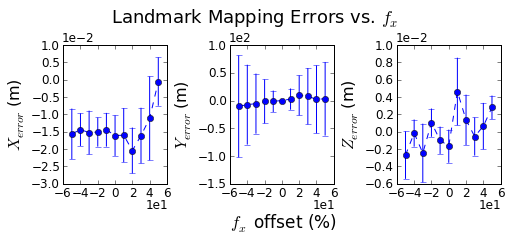
\includegraphics[width=10cm,keepaspectratio=true]{./Figures/SimulationFigures/Figure38.png}
  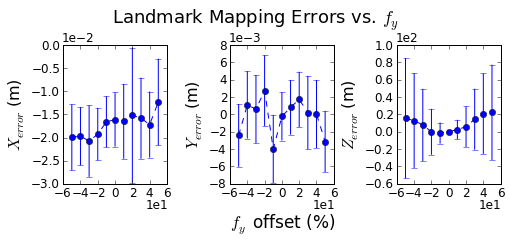
\includegraphics[width=10cm,keepaspectratio=true]{./Figures/SimulationFigures/Figure39.png}
  \caption{Landmarks mapping errors statistics with variable $(f_x, f_y)$}
  \label{fig:simfig38-39}
\end{figure}

Plotting the landmarks mapping errors against landmarks ground truth
positions also showed that the mapping errors were dependable on
landmarks ground truth positions and error in $(f_x, f_y)$. When $f_x$
contained error, landmarks positions errors on Y were directly
proportional to the Y component of their ground truth positions, with the
error in $f_x$ determining the steepness of the slope. Same relation can be
found for $Z_{error}$ with $f_y$, and $Z_{ground truth}$.

\begin{figure}[h]
  \centering
  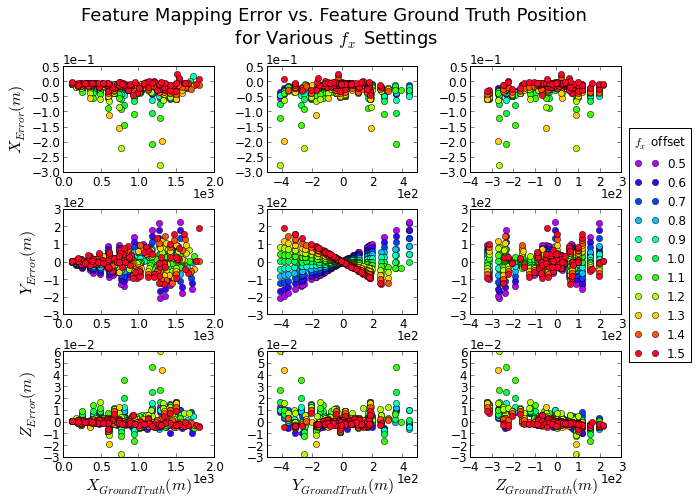
\includegraphics[width=13cm,keepaspectratio=true]{./Figures/SimulationFigures/Figure41.png}
  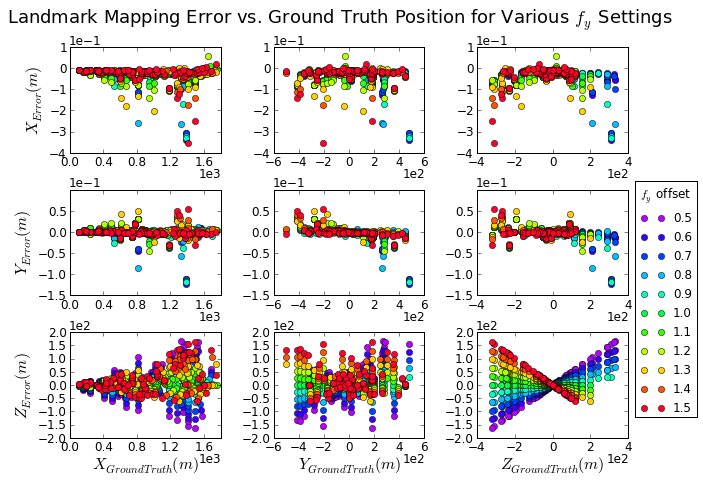
\includegraphics[width=13cm,keepaspectratio=true]{./Figures/SimulationFigures/Figure42.png}
  \caption{Landmarks mapping errors plotted against ground truth
    for various $(f_x, f_y)$}
  \label{fig:simfig38-39}
\end{figure}
\FloatBarrier

\subsection{Effect from Distortion}
% word checked.
The CC\_EKF\_SLAM algorithm did not consider camera lens distortion
at this stage. Therefore, the simulation evaluated the effect of
lens distortion varying from 0\% to 150\% of the base value to
estimate the amount of error resulted from ignoring the lens distortion.

Figure \ref{fig:simfig47} showed the UAV localization error for
various lens distortion setting. Ignoring the distortion brought
significant error into the UAV localization. UAV position on X-axis
received the most impact. The errors were up to 100 meters, and with
increasing standard deviation. Positions on Y and Z axes showed less
error, but standard deviation grew  larger with the increasing amount of
distortion added. 

Figure \ref{fig:simfig48} revealed the cause of increasing standard
deviation. UAV position errors were diverging in time and with amount
of lens distortion added. UAV orientation errors increased from
maximum mean error of 5e-6 radius in low noise simulation to 2.5e-4
rad. Similar to position error, the plots of orientation error vs.
frame number showed that the error amplitude increases with time,
but it fluctuated around zero.

\begin{figure}[h]
  \centering
  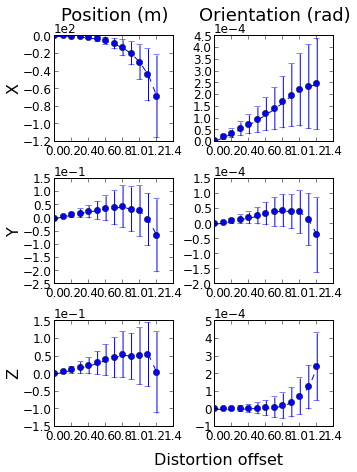
\includegraphics[width=10cm,keepaspectratio=true]{./Figures/SimulationFigures/Figure47.png}
  \caption{UAV localization errors statistics with lens distortion}
  \label{fig:simfig47}
\end{figure}

\begin{figure}[h]
  \centering
  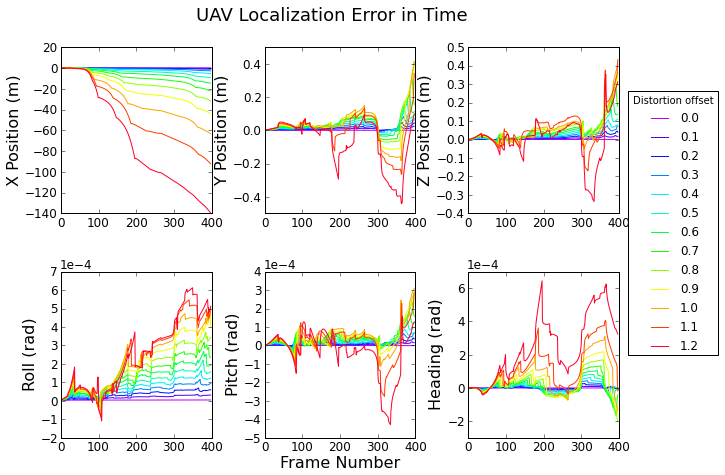
\includegraphics[width=14cm,keepaspectratio=true]{./Figures/SimulationFigures/Figure48.png}
  \caption{UAV localization error plots with lens distortion}
  \label{fig:simfig48}
\end{figure}

The landmarks positions errors statistics were shown in figure
\ref{fig:simfig45}. The positions errors were also plotted against
landmark ground truth positions in figure \ref{fig:simfig46}. The
landmarks positions on X axis showed the most error, with mean error
at -400 meters with distortion offset at 120\%. The amount of error
was related to the landmarks' distance from X axis (Figure
\ref{fig:simfig46}, subplots [1,2] and [1,3]). The further the
landmarks lied away from the X axis, the bigger the errors became.
Landmarks positions on Y, and Z axes had less mean error, but the
standard deviation were bigger. Figure \ref{fig:simfig46} subplots
[2,2] and [3,3] showed that the errors on Y (or Z) axes were loosely
proportional to the landmarks ground truth coordinates on Y (or Z)
axis, where distortion offset determined the slope of the line. The
relation indicated that landmarks lying around the sides of the image
plane carried more errors than landmarks at the center of the image on
all axes. This was exactly the kind of error that radial distortion
corrected for.

\begin{figure}[h]% get rid of title and reposition x label
  \centering
  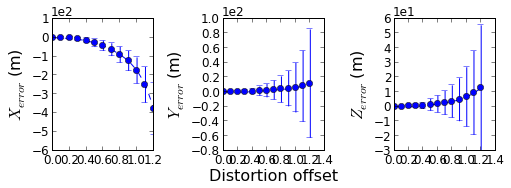
\includegraphics[width=10cm,keepaspectratio=true]{./Figures/SimulationFigures/Figure45.png}
  \caption{Landmarks positions errors with lens distortion}
  \label{fig:simfig45}
\end{figure}

\begin{figure}[h] %get rid of the title. 
  \centering
  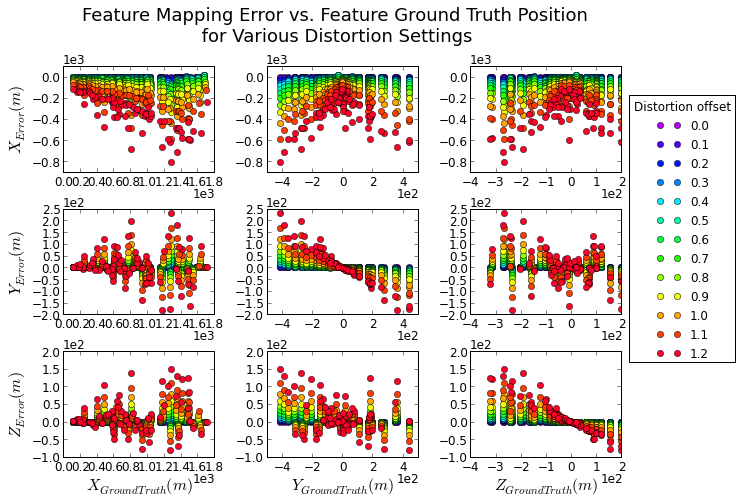
\includegraphics[width=13cm,keepaspectratio=true]{./Figures/SimulationFigures/Figure46.png}
  \caption{Landmarks positions errors vs. ground truth positions with lens distortion}
  \label{fig:simfig46}
\end{figure}
\FloatBarrier

\subsection{Effect from Image Resolution}

It is well known that higher resolution sensors give more accuracy
to the estimates. To know how high a resolution is good enough for the
distance that this research was targeting at, a quantitative
analysis was necessary. A few simulations were ran with various image
resolution settings, and the results were shown in figure
\ref{fig:simfig50}.

%TODO regenerate top figure to give enough room for xlabel, change UAS
%to UAV
\begin{figure}[h] 
  \centering
  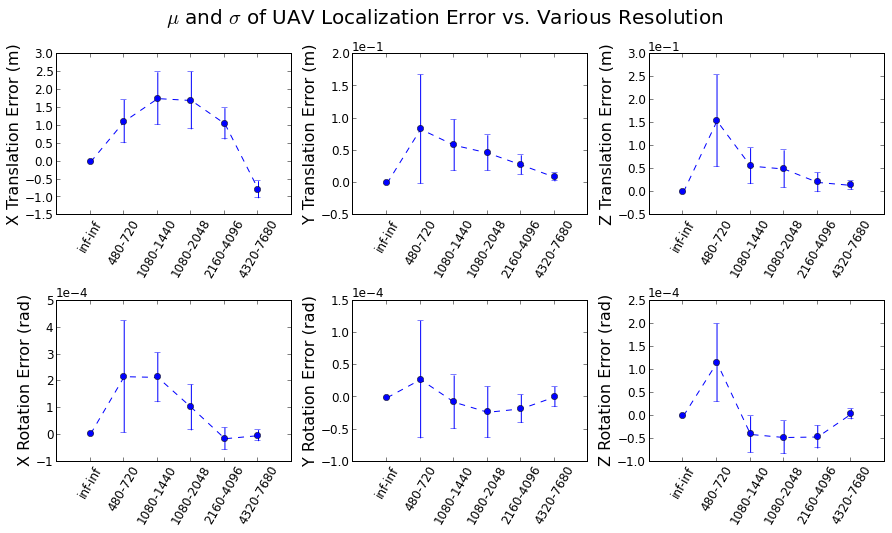
\includegraphics[width=10cm,keepaspectratio=true]{./Figures/SimulationFigures/Figure50.png}
  \caption{Localization errors statistics for various image resolution}
  \label{fig:simfig50}
\end{figure}

\begin{figure}[h] % regenerate to make room for x axis label. change
                  % feature to landmark
  \centering
  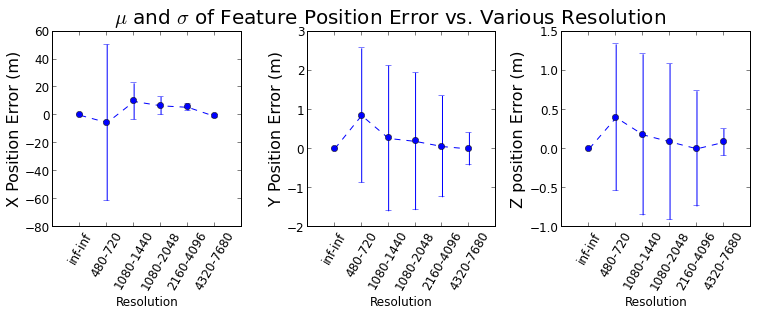
\includegraphics[width=10cm,keepaspectratio=true]{./Figures/SimulationFigures/Figure49.png}
  \caption{Landmarks mapping errors statistics for various image resolution}
  \label{fig:simfig51}
\end{figure}

This test confirmed that the higher resolution the image sensor had,
the more accuracy it would bring. The most significant error was seen
at resolution 480x720 where the landmarks positions errors on X were
+/- 150m. At 720x1080, the X axis landmarks positions errors were
greatly reduced to a few meters. For all other parameters,
improvements at each level of resolution increase were nearly linear.
This result suggested that to achieve reasonably good accuracy for
obstacle detection, a sensor with resolution of 720x1080 or higher is
preferred.


%%% Local Variables:
%%% mode: latex
%%% TeX-master: "thesis"
%%% End:
